\Chapter{Implementation}
Taking into consideration the language specific elements, we must construct the three main parts, namely the lexer, parser and engine, in such a way to make their operations and interactions smooth. The different algorithms and processes to analyze text, parse tokens and calculate the states is explained via pseudo code and, in some cases, with the help of code snippets from the interpreter.

\Section{Lexical Analyzer}
The first stage in the program is the lexical analysis, also called tokenization, a process which dissects and ``categorizes'' the input based on some predefined rule and extracts a stream of tokens, or in this case the \textit{getNextToken} function returns them one by one at each call. Everything else that is not needed or does not carry meaningful information is discarded such as white spaces, tabs, newline character, or any type of control character and only the allowed tokens are processed.

Upon receiving a call the function must first \textit{trim} the input, simply skip the characters which are of no use to us such as all the control characters and those outside the alphanumeric range. Note that whenever we iterate over the input extensive checks are necessary in order to mitigate any indexing related issues.

\begin{octave}
function lexer = trim (lexer)
  while lexer.cursor <= lexer.content_len &&
  ((lexer.content(lexer.cursor) < 33) ||
  (lexer.content(lexer.cursor) == 127))
    if lexer.content(lexer.cursor) == "\n"
      lexer.line++;
      lexer.beginning_of_line = lexer.cursor;
    end
    lexer.cursor++;
  end
end
\end{octave}

Then we must determine if we have run into a comment line, marked by a \textit{\# (hashtag)} symbol or reached the end of the file. In the case of the former, we treat it in a similar manner to trimming, but only going until a \textit{\\n (newline} character is reached, whilst regarding the latter, a token is emitted with type \textit{EOF} and no value.

Now we can finally start examining whether the stream of characters read from the input are part of an accepted token. Since we read individual characters from the input it is not possible to tell if it is going to be a valid token until we have read the whole word, however just from the first character we can categorize it as a possible token and then hand the procedure for checking to the appropriate function. In a case where an invalid character sequence is encountered the program raises a syntax error with the appropriate message and also displays the line and column numbers where the fault occurred, then exits.

\SubSection{Identifier (reserved)}
An identifier may start with an underscore or any letter from the English alphabet found in the ASCII character set; case sensitivity is not considered. Characters apart from the first one can include numbers as well. Since no functionality for handling identifiers are currently implemented in the latest version of the interpreter, and neither in the grammar of the FBDL, only keywords are permitted in the supplied FBDL source code. However given the similarity of lexical analysis in both cases some room has been left for possible accommodation of this feature at a later time.

After a token is read as an identifier its value is compared against the list of available keywords, if a match is found the token type is changed to keyword and returned.

\begin{octave}
...
while lexer.cursor <= lexer.content_len &&
		isIdent(lexer.content(lexer.cursor))
  lexer.cursor++;
end
token.value = substr(lexer.content, lexer.token_begins,
		lexer.cursor - lexer.token_begins);
if any(strcmp(lexer.keywords, token.value))
  token.type = "keyword";
end
...
\end{octave}

The list of keywords may be extended or have entries removed, granted the modification is permitted by the grammar of the language. This is the case with the \textit{dominates} keyword as hierarchical rule dominance is not implemented in the program, but is found in the grammar as an optional language element.

\SubSection{Terminal (reserved)}
Similarly to identifiers it is not yet available in the FBDL grammar, but some consideration has been taken to allow for future extensions that include these elements.

\SubSection{String}
Encountering a '' (double quote) symbol implies that a string will follow and accordingly every character is skipped until the closing pair is not reached. The lexer holds every token's starting position, in this particular case that happens to coincide with the position of the double quote at the beginning, which will later be used as an index to copy the contents of the string and store it in a token. This procedure is used in case of every token that has a value.

The length of a given string is unknown when iterating over it, the only way to see if it is invalid, or in other words the closing double quotes are missing, is to see if we have reached the end-of-file beyond which there cannot be any more characters. Empty strings are permitted and no value copying happens in such a case.

Escape characters are not yet allowed in strings and there are no implementations to process them, they are simple copied as literal characters just as the rest of the string.

With extended Backus-Naur form :
\begin{grammar}
<string> ::= '' character* ''
\end{grammar}

\SubSection{Number}
The first thing to consider when checking for numerical constants is the presence of the optional negative sign, since it is not itself a numerical value, most often being denoted with a \textit{- (dash)}. The absence of such a sign implicitly implies a positive number, therefore the need for a \textit{+ (plus)} sign is eliminated and is not processed. Then a series of numbers, digits, must follow until the end of the token; the very first digit cannot be zero. Every number may contain a single negative sign before the first digit and a single decimal point between two adjacent digits marked by a \textit{. (dot)} character. Failing to meet any of these conditions will result in a syntactical error being raised and the program exiting. Although floating point numbers are accepted, their syntactical version of scientific notation is not; furthermore the language does not support arbitrary-precision arithmetic.

After passing these checks the series of digits is copied from the input text and is converted to a double precision floating point type, which is then returned in the token. This step allows direct referencing of the token's value during calculations in the engine without needing to do the conversion there.

With extended Backus-Naur form:
\begin{grammar}
<number> ::=  [-]  (integer | fraction)

<integer> ::= digit-z+ digit*

<fraction> ::= (integer | 0) `.' digit*

<digit> ::= 0 | digit-z

<digit-z> ::= 1 | 2 | 3 | 4 | 5 | 6 | 7 | 8 | 9

\end{grammar}

\Section{Parser}
Every language conforms to some form of grammatical rule base from which it cannot deviate, otherwise it would not be valid. The grammar employed by the FBDL has been mentioned before and now the part that is responsible for the correct interpretation of code that uses said grammar will be explained. The interpreter makes use of a technique called \textit{recursive descent top-down parsing} \cite{burge1975}\cite{aho1986}, where every non-terminal in the grammar is handled by a dedicated function. In this section each rule within the grammar will be compared against the code of the parser to see its method of operation and also note some problems which often makes the process more complicated than necessary. Since the actual implementation of each function is quite lengthy, it is most adequate to demonstrate only the underlying logic via pseudo code.

The very first rule is straightforward, stating that there must be at least 1 occurrence with regards to the \textit{universe} and \textit{rulebase}. The \textit{init} optional part is not implemented in the program, therefore it will be skipped.
\begin{grammar}
<behavior> ::= universe+ rulebase+ [init]

<universe> ::= `universe' string [`description' string] symbol+ `end'

<symbol> ::= string number number
\end{grammar}

Every language construct besides terminals and the first rule is enclosed between two keywords, namely the one indicating what object it is defining and an \textit{end} keyword. The \textit{universe} requires a name of type string and a series of symbols, which will define the variables and their range of values for later usage. Despite an optional description being available in the grammar, this and all such options in the following rules are yet to be implemented and therefore no algorithm is given for the procedure.

\vskip 0.5cm
\begin{algorithm}[H]
	\KwResult{Universe:}
	\If{token is literal}{
		universe.name = token.value\;
		check optional description\;
		next token\;
		\While{token is literal}{
			symbol.name = token.value\;
			next token\;
			\If{token is number}{
				symbol.position = token.value\;
			}
			next token\;
			\If{token is number}{
				symbol.value = token.value\;
			}
			next token\;
		}
		\If{keyword is 'end'}{
			universe += symbol\;
			return universe\;
		}
	}
\caption{Parsing the \textit{universe}}
\label{fig:parseuniverse}
\end{algorithm}
\vskip 0.5cm

Implementation and language specific elements have been eliminated or reduced as much as possible for clarity in figure \ref{fig:parseuniverse}, furthermore all checks and error messages have been omitted in order to provide the minimal code required while preserving its semantic integrity. Similar simplifications will be used for all demonstrations to keep the focus on understanding the algorithm rather than being lost in obscure syntax.

With that said the next rule is concerned with the \textit{rulebase}, which is almost identical to the \textit{universe} only differing in the containment of a series \textit{rule} elements as opposed to \textit{symbols}.
\begin{grammar}
<rulebase> ::= `rulebase' string [`description' string] rules `end'

<rules> ::= rule+
\end{grammar}

However, these rules require an algorithm much more complicated than in the case of the previous grammar rules.
\begin{grammar}
<rule> ::= `rule' [`description' string] [`use'] string [`when' predicates] `end'

<predicates> ::= predicate (`and' predicate)*

<predicate> ::= string `is' string
\end{grammar}

Once again, as observed on figure \ref{parserule}, discarding the first optional argument, the \textit{use} keyword references the value of a previously calculated variable and is further used  in calculating behavior fusion resulting from all other behavior components, i.e. rule-bases.

\vskip 0.6cm
\begin{algorithm}[H]
	\KwResult{Rule:}
	\uIf{token is literal or keyword}{
		read optional arguments\;
		next token\;
		\If{token is `when' keyword}{
			read predicates\;
		}
	}
	\uElseIf{token is not `end' keyword}{
		error\;
	}
	\Else{
		error\;
	}
\caption{Parsing a \textit{rule}}
\label{fig:parserule}
\end{algorithm}
\vskip 0.6cm

These two algorithms occupy the same function, but to avoid any ambiguity they have been presented as separate. In the case of every grammar rule the checking of enclosing keywords is paramount along with other type checks as well. Encountering a problem, as denoted by \textit{error},  at any point in these functions will result in the program exiting and returning an appropriate error message.

\vskip 0.6cm
\begin{algorithm}[H]
	\KwResult{Predicates:}
	\While{token is not `end'}{
		next token\;
		\If{token is literal}{
			antecedent = token.value\;
		}
		next token\;
		\If{token is  not `is' keyword}{
			error\;
		}
		next token\;
		\If{token is literal}{
			value = token.value\;
		}
		next token\;
	
		\If{antecedent already in predicates}{
			error\;
		}
		next token\;
		\If{token is neither `and' nor `end' keyword}{
			error\;
		}
	}
\caption{Parsing the \textit{predicates}}
\label{fig:parsepred}
\end{algorithm}
\vskip 0.6cm

The series of predicates is processed in the same manner is the \textit{symbols} from before, albeit with a longer algorithm, seen in figure \ref{fig:parsepred}. Furthermore in case any antecedent is already present in the list of predicates, in other words, it is a duplicate predicate, an error is raised.

After the parsing of the input stream is completed additional semantic checks are required to ensure that the variables used within rules conform to previous definitions regarding names and values; the same applies to the rules themselves, including the predicates.

\begin{octave}
function checkRulebaseNames(behavior)
  len = length(behavior.rulebases);
  if len == 0
    error("Parse error! At least one rulebase must exist!\n")
  end

  for i = 1:len
    if !isfield(behavior.universes, behavior.rulebases(i).name)
      error("Parse error! Missing universe definition for rulebase\n");
    end
  end
end
\end{octave}

If any part of a given rule, regardless of being a consequent or an antecedent, is not presented in the universe, then it is reported as an error, since it has not been previously defined.
\begin{octave}
function checkRulebaseRules(behavior)
  for i = 1:length(behavior.rulebases)
    rulebase = behavior.rulebases(i);
    for j = 1:length(rulebase.rules)
      rule = rulebase.rules(j);
      checkRule(rulebase.name, rule, behavior.universes);
    end
  end
end
\end{octave}

\Section{Engine}
At the last stage of the operation is a direct implementation of the previously mentioned Fuzzy Automaton mathematical model, that performs all the necessary calculations required for simulating fuzzy behaviour. The entire system is a state machine, meaning that the initial values of the variables inside the universe will be used in the first and then subsequent transitions, and are subject to change as the automaton moves from one state to another.

Similarly to the lexical analysis stage an \textit{engine} object is created at the beginning, which holds the syntax tree and also contains additional information such as the state of each variable, distance values and other elements as well. This structure is passed around by functions that use these data to calculate various intermediate variables for later determining the state transition of each variable. For easier referencing during processing the states and collection of antecedents are gathered and stored in a list. In the next step, the integrity of these initial variables are checked and they must conform to the following conditions:

\begin{itemize}
	\item All universes listed must be defined.
	\item The symbol values of a given universe must be bounded by the universe.
	\item All input values must be defined.
\end{itemize}

As these are initial values the user of the interpreter can modify any of their parameters, name the values of variables, to fit their need or simply experiment.

Next, we must evaluate the consequents, but before that, it is required to calculate the distance of observations from the symbols on every antecedent universe. As listed by the example from \cite{pillerkovacs2019}, considering the following universes and initial values defined:

\begin{fbdl}
universe "distance"
  "zero" 0 0
  "close" 1 0.1
  "far" 5 1
  "max" 10 1
end
\end{fbdl}

\begin{fbdl}
universe "curiosity"
  "low" 0 0
  "high" 1 1
end
\end{fbdl}

\begin{fbdl}
universe "speed" 
  "low" 0 0 
  "high" 1 100 
end 
\end{fbdl}

\begin{fbdl}
init
  "distance" 3
  "curiosity" 0.4
end
\end{fbdl}

\noindent In the distance universe example above the consequent value lies on the $[0, 1]$ interval. Distance values above 5 are treated the same; anything larger up to 10 is considered ``far''.
We also define a set of rules:

\begin{fbdl}
rulebase "speed" 
  rule "high" when "distance" is "far" and "curiosity" is "high" end 
  rule "low" when "distance" is "close" end 
  rule "low" when "curiosity" is "low" end 
end
\end{fbdl}

Considering the first rule, we must calculate the distance of 3 from ``far" in the ``distance” universe. The distance is determined from the difference of the cumulative scaling function values of the two points. That is, the value of the cumulative scaling function at 3 is 0.55 and at ``far” it takes the value 1, therefore their cumulative scaled distance is 0.45. Similarly we can calculate the distance of 0.4 and “high” on the “curiosity” interval resulting in the value 6. The distance of the rule is given by the Euclidean norm of the distances by dimensions divided by the square of the number of antecedents.

The rule distance for the first rule can be calculated in the following manner:
\[
	d_{rule1} = \frac{\sqrt{0.45^2 + 0.6^2}}{\sqrt{2}} \approx 0.5303.
\]
\noindent The other two rules are computed in the same way:
\[
	d_{rule2} = \frac{\sqrt{0.45^2}}{\sqrt{2}} \approx 0.3182,
	d_{rule3} = \frac{\sqrt{0.4^2}}{\sqrt{2}} \approx 0.2828.
\]

If the distance from some rules is 0, then the consequent is calculated as the \textit{mean value} of the corresponding consequent symbol values, or variable values. The weights are the reciprocals of the distances raised to the Shepard-power $p$, so that $w_i = \frac{1}{d^p_i}$.

\noindent If $p = 1$, then the weights of the rules are respectively:
 \[
 	w = 1.8856, 3.1427, 3.5355.
 \]

\noindent The consequent values of the rules are:
\[
	c = 1, 0, 0.
\]

\noindent The consequence can be obtained as the sum of weighted rule consequents, using the rule weights:

\[
	C = \frac{\sum_i w_i  c_i}{\sum_i w_i} \approx \frac{1.8856}{8.5638} \approx 0.2202.
\]

\noindent The consequent value of the “speed” rule-base is approximately 22.0183. 

Seen on figure \ref{fig:example} is a model of the interactions between universes, rules and consequents.
\begin{figure}[!h]
	\centering
	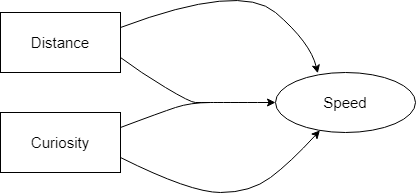
\includegraphics[width=0.6\textwidth]{images/example}
	\caption{Evaluation of rule-bases}
	\label{fig:example}
\end{figure}

\Section{Error Handling}
Upon encountering an error, the program should terminate its operations immediately, report the fault with informative messages and then exit gracefully. A ``token" based method was considered before to check the integrity of operations; in response to catching an error a special token would be emitted and since the top-most function is the one receiving these tokens, specifically the parser, it should be the one to terminate the program. However the probability of errors occurring is numerous and creating tokens at every one of these places is neither a space efficient nor a logically sound approach, leading to much confusion and clutter. The preferred method chosen was using the \textit{error(msg)} function both found in Octave and MATLAB, where a message \textit{msg} would also be displayed to the user. Calling the function directly is not appropriate, since not only the fault needs to be reported, but its position as well. Furthermore to facilitate the process of locating the problematic section of code resulting in the error, the whole line where the program failed is printed to the screen.

\begin{octave}
function raiseError (lexer, type, msg)
  while (lexer.cursor <= lexer.content_len &&
       lexer.content(lexer.cursor) != "\n")
    lexer.cursor++;
  end

  snippet = substr(lexer.content,
  lexer.beginning_of_line, lexer.cursor - lexer.beginning_of_line);
  error("%s! At line %d, column %d!\n%s\n%s\n",
    type, lexer.line, lexer.cursor - lexer.beginning_of_line,
    msg, snippet);
end
\end{octave}


\Section{Future Extensions}
With time programming languages usually evolve, and the FBDL is no exception, therefore, it is quite sensible to employ an architecture that is capable of adapting to changes in code and also leaves room for extensions. Various elements in the language such as strings, numbers, terminals and keywords or even grammar are susceptible to change. Regarding the first in the list, strings might contain escape characters and as such the \textit{lexer} must store a list of characters that are accepted as valid escape sequences and during the parsing of strings correctly map them to the given control character. Number definitions could also include scientific notation or perhaps even complex numbers, although the benefits of the latter are not obvious to me. Implementing functions would require the modification of the grammar and also introducing new elements to parsing, namely identifiers and terminals, hence the main reason they are considered reserved.

In the case of the parser, the processing of optional arguments should be implemented at some point in the future along with warning messages, when they are missing. In the original paper \cite{pillerkovacs2015}, a hierarchical implementation of rules is also defined with the help of the \textit{dominates} keyword, which also ought to be interpreted correctly to work with multiple, highly interconnected rules. With regards to numbers once more, currently only numerical constants are accepted as valid values, but should the need arise for them to be replaced with mathematical expressions, then new parsing techniques would also be required, namely precedence climbing, in order to handle these cases.

More advanced techniques may be integrated into the engine to process these rules more efficiently. Since each rules if independent of one another this presents a massively parallel environment, which is beneficial during the scaling of the model. Other types of interpolation methods could be employed and examined to see if the produce different results.

Although these possible extensions mentioned might evoke optimism for broadening the language, a fundamental property would be lost in the process, that being its simplicity. Therefore one should carefully consider before any significant alteration to the language what is to be gained with these additions of ``tools" and what is to be lost.